\documentclass[apjl]{emulateapj}

\usepackage{hyperref}
\usepackage{amsmath}
\usepackage{amssymb}
\usepackage{graphicx}
\usepackage{color}
\usepackage{natbib}

\newcommand{\MSun}{M_\odot}
\newcommand{\RSun}{R_\odot}
\newcommand{\Rstar}{R_*}
\newcommand{\Mstar}{m_*}
\newcommand{\MBH}{M_\mathrm{BH}}

\def\aj{Astronomical Journal}                 % Astronomical Journal
\def\apj{Astrophysical Journal}                % Astrophysical Journal
\def\apjl{Astrophysical Journal}             % Astrophysical Journal, Letters
\def\pasj{PASJ}
\def\apjs{ApJS}              % Astrophysical Journal, Supplement
\def\mnras{MNRAS}            % Monthly Notices of the RAS
\def\prd{Phys.~Rev.~D}       % Physical Review D
\def\prl{Phys.~Rev.~Lett}    % Physical Review Letters
\def\cqg{Class.~Quant.~Grav.~}%Classical and Quantum Gravity
\def\araa{ARA\&A}             % Annual Review of Astron and Astrophys
\def\nat{Nature}              % Nature
\def\aap{A\&A}                % Astronomy and Astrophysics
\def\na{New Astronomy}

\newcommand{\will}[1]{\textcolor{cyan}{#1}}
\newcommand{\ilya}[1]{\textcolor{red}{#1}}

\newcommand{\onesigrange}[3]{\ensuremath{#1^{+#2}_{-#3}}}
\newcommand{\alpharangeone}{\onesigrange{2.05}{0.14}{0.12}}
\newcommand{\alpharangetwo}{\onesigrange{2.13}{0.13}{0.13}}
\newcommand{\alpharangethree}{\onesigrange{2.22}{0.17}{0.16}}
\newcommand{\alpharangefour}{\onesigrange{2.68}{0.23}{0.21}}

\begin{document}

\title{Comment on ``An excess of massive stars in the local 30 Doradus starburst''}

\author{Will M. Farr\altaffilmark{1}, Ilya Mandel\altaffilmark{1}}
\affil{$^1$Institute of Gravitational Wave Astronomy and School of Physics and Astronomy, University of Birmingham, Birmingham, B15 2TT, United Kingdom}
\email{wmfarr@star.sr.bham.ac.uk, imandel@star.sr.bham.ac.uk}

\begin{abstract}
Schneider et al.~(Reports, 5 January 2018, p.~69) found more stars above 30 solar masses than predicted by a standard Salpeter initial mass function (IMF) in the 30 Doradus star-forming region.  Their finding of an IMF power-law exponent of $1.90^{+0.37}_{-0.26}$ is based on a flawed statistical analysis of the data and a number of uncertain assumptions.  We discuss the uncertainties and re-analyze their data to find a preferred IMF exponent of $\alpharangethree$, consistent with the Salpeter value of $2.35$.  We also discuss a number of modelling choices that can shift the exponent to steeper or shallower values.
\end{abstract}

\maketitle

The universality of the initial mass function of stars is a hot topic in modern astrophysics, with impact on galactic evolution, supernovae, and gravitational-wave sources \citep{Kroupa:2002,Bastian:2010,deMinkBelczynski:2015}.    \citet{Schneider:2018} use spectroscopic observations of young massive stars in the 30 Doradus region of the Large Magellanic Cloud to infer a shallower-than-expected IMF.  Their conclusion is due to a faulty statistical methodology and several questionable assumptions which we discuss below.

\citet{Schneider:2018} obtain estimates of the ages and masses of individual stars with the BONNSAI Bayesian code \citep{Schneider:2017}.  They then obtain an overall mass distribution by effectively adding together the posterior probability density functions of individual stars.  There is no statistical meaning to a distribution obtained in this way, and it does not represent the posterior probability density function on the underlying mass distribution.  %In fact, when the underlying distribution is a steeply decaying power law, as considered here, the approach of \citet{Schneider:2018} will yield a distribution biased toward the high-mass end.  The measurement uncertainty will ``smear out'' the masses of both low-mass and high-mass stars, but because there are far more low-mass stars than high-mass ones, this appears to yield more mass at the high end of the distribution, leading to a false conclusion of a shallower distribution.

Hierarchical Bayesian inference provides the statistically correct solution to
this problem \citep{Hogg:2010}.  \citet{Mandel:2010stat} specifically considered
inference on a mass distribution given a sample of uncertain measurements, and
we use this methodology here.  We interpret their inference
on individual masses and ages as independent Gaussian likelihoods for the log
of the mass and the age, with parameters fixed by matching the mean parameter to the peak and the standard deviation parameter to the 68\% width of the
individual stellar distributions in the \citet{Schneider:2018} data.  We have performed fits similar to those described here using a heavier-tailed, Student T likelihood with few degrees of freedom and find equivalent results, suggesting that heavy tails in the likelihood are not particularly influential in this analysis.

We model the star formation history as a truncated Gaussian distribution, and
generally find similar star formation history to \citet{Schneider:2018}, with
the star formation rate peaking in 30 Dor about 4 Mya.  We impose broad priors
on the power--law exponent and the mean and standard deviation of the star
formation Gaussian.    We use the Hamiltonian Monte Carlo sampler STAN
\citep{STAN} to efficiently address the high-dimensional hierarchical problem
with free parameters for each star's actual mass and birth age in addition to
the IMF exponent and the mean and standard deviation of the star formation
history.

Figure \ref{fig:IMF} shows the inferred power-law exponent of the IMF.   When
using the full data set of \citet{Schneider:2018}, following their assumption
that their data set is complete above 15 solar masses, and using their fit to
stellar lifetimes, we find an exponent of $\alpharangeone$ where the quoted
value corresponds to the median of the posterior distribution and the range to
the 16th and 84th percentiles (i.e.\ the symmetric 68\% credible interval).  
Correcting the erroneous statistical procedure used by \citet{Schneider:2018}
steepens the preferred IMF slope and narrows the uncertainty interval; the
preferred value from \citet{Schneider:2018} lies about $1\, \sigma$ below our
median value.

The analysis above used the same assumptions as \citet{Schneider:2018}.  Below, we consider the impact of three additional questionable assumptions: the stellar lifetime fit; the choice of the completeness limit; and the inclusion of stars for which limited measurements are available.

The fit to stellar lifetimes used by \citet{Schneider:2018} continues to
decrease at high masses, in contrast to the expectation that stellar lifetimes
should asymptote to a fixed minimum duration for high-mass stars set by the
ratio of the energy to be released through nuclear fusion to the Eddington
luminosity.  We make an independent fit to the main sequence lifetimes
$\tau_{MS}$ of non-rotating massive stars as modelled by \citet{Brott:2011} (in
our fits, following \citet{Schneider:2018}, we increase the ``observable''
lifetime of a star by 10\% beyond its main sequence lifetime to account for
helium burning):
%
\begin{multline}
\ln \frac{\tau_{MS} (M)}{\textrm{Myr}} = 9.604 - 4.196 \log\frac{M}{M_\odot} \\ + 0.671 \left(\log\frac{M}{M_\odot} \right)^2 - 0.036 \left(\log\frac{M}{M_\odot}\right)^3.
\end{multline}
%
Our fit predicts longer lifetimes for stars more massive than $\sim 100 M_\odot$
than the \citet{Schneider:2018} fit.  Using our fit rather than the
\citet{Schneider:2018} fit therefore leads to a steeper power-law exponent,
$\alpharangetwo$, as there are fewer massive stars that should have already
collapsed into invisible remnants in our model.

The inferred power-law exponent is somewhat sensitive to
the choice of the cutoff mass for survey completeness.  The data of \citet{Schneider:2018} show a relative scarcity of stars between 15 and 20 solar masses; changing the mass cutoff from $15 M_\odot$ to $20 M_\odot$ further steepens the inferred exponent to $\alpharangethree$.    However, these fluctuations are within the expected statistical
variation based on the sample size, as confirmed with posterior predictive
checking.  In particular, we do not claim statistical evidence against the claim of \citet{Schneider:2018} that
the survey is complete for $M \geq 15 \, \MSun$.

Finally, we note that $13$ stars in the \citet{Schneider:2018} data set are
missing one or both $\log g$ and $T_\textrm{eff}$ measurements.  We
conservatively remove these stars from the analysis, as their mass and age
estimates may be particularly uncertain.  Inference on this reduced data set
yields an even lower estimate of the power-law exponent $\alpharangefour$ as
the removed stars have high estimated masses.

\begin{figure}
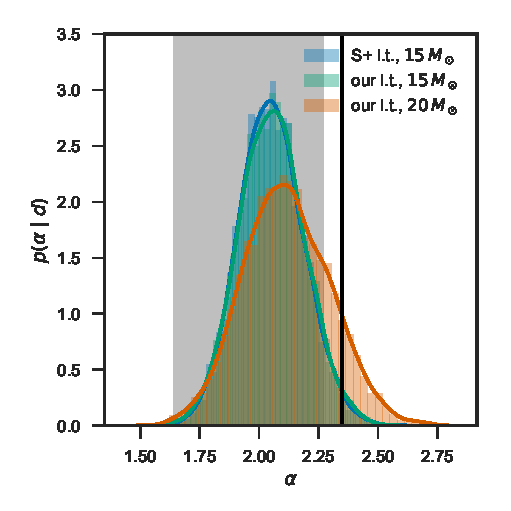
\includegraphics[width=\columnwidth]{alpha.pdf}
    		\caption{The posterior inferred on the power-law exponent under four models (see text for details): \citet{Schneider:2018} stellar lifetimes, survey completeness for $M \geq 15 \, \MSun$, and full \citet{Schneider:2018} data set (blue); as before, but with our lifetime fit (green); as before, but with completeness for $M \geq 20 \, \MSun$ (orange); as before, but with stars without $\log g$ and $T_\textrm{eff}$ measurements removed (pink).  The Salpeter power-law exponent is $-\alpha=-2.35$ \citep{Salpeter:1955}, indicated by a black line.  The 68.3\% range of power-law exponents derived by \citet{Schneider:2018} is shaded in grey. }\label{fig:IMF}
\end{figure}

We confirm the stability of our conclusions with posterior predictive checking.
Figure \ref{fig:PPC} shows the distribution of observed masses and ages (i.e.,
the peak of the likelihood) from the \citet{Schneider:2018} data on top of the
range of mass and age distributions that would be observed from a large number
of data sets drawn according to our fitted IMF model.  The data can be seen to
be consistent with our IMF model.  We have also confirmed that all of our models yield predictions for the numbers of stars heavier than $30 M_\odot$ and $60 M_\odot$ that are consistent with observations.

\begin{figure}
%\vspace{-1in}
    		    		\includegraphics[width=\columnwidth]{dNdm-ppc-band.pdf}\\
                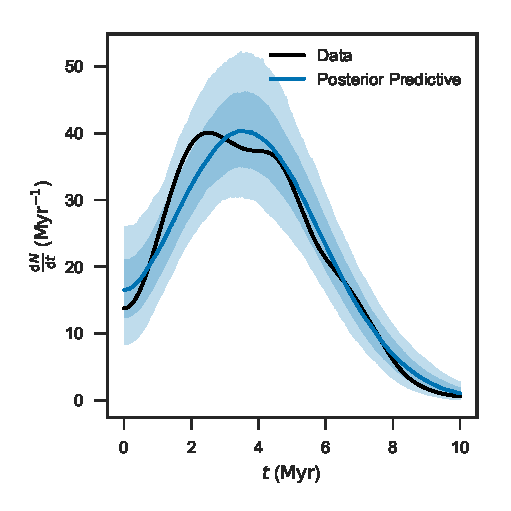
\includegraphics[width=\columnwidth]{dNdt-ppc-band.pdf}
%\vspace{-1in}
    		\caption{The observed distribution of (maximum likelihood) masses (top, black) and ages (bottom, black) and the range (median, 68\%, and 95\% credible intervals in blue) of distributions of mass and age from synthetic data drawn from our fitted model (i.e.\ the posterior predictive distribution).  The observed data are consistent with being drawn from our model.  %We see no evidence that our model is unable to account for the features in the observed data, including the apparent shallowing of the exponent of the mass distribution for $M \gtrsim 60 \, \MSun$.
		}\label{fig:PPC}
\end{figure}


In conclusion, we find that there is no significant evidence for a deviation from the Salpeter IMF \citep{Salpeter:1955} in the observations of young massive stars in 30 Doradus once the correct statistical analysis is applied and uncertainties in stellar lifetimes and selection biases are accounted for.

\acknowledgments

%While this note is critical of the conclusions in \citet{Schneider:2018}, those authors should be
We are grateful to \citet{Schneider:2018} for making the data on which their conclusions are
based available for further study and analysis, and to Fabian Schneider personally for very useful discussions.  This analysis made use of \texttt{PySTAN} \citep{PySTAN}, \texttt{astropy} \citep{astropy}, \texttt{numpy} \citep{numpy}, \texttt{scipy} \citep{scipy}, \texttt{matplotlib} \citep{matplotlib}, and \texttt{seaborn} \citep{seaborn} Python libraries.  The code and \LaTeX source used to prepare this document are publicly available under an open-source MIT license at \url{https://github.com/farr/30DorIMF}.  WMF and IM are partially supported by STFC.

\bibliographystyle{hapj}
\bibliography{Mandel}
\end{document}
